\documentclass[
%% TIKZ_CLASSOPTION %%
tikz
]{standalone}
\usepackage{amsmath}
\usetikzlibrary{matrix}
%% EXTRA_TIKZ_PREAMBLE_CODE %%
\begin{document}
%% TIKZ_CODE %%
\usetikzlibrary{positioning}
\usetikzlibrary{shapes.geometric}
\usetikzlibrary{arrows}
\usetikzlibrary{decorations}
\tikzstyle{Arrow} = [->, thin, preaction = {decorate}]
\tikzset{>=latex}

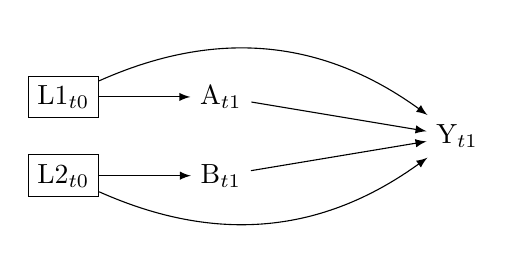
\begin{tikzpicture}[{every node/.append style}=draw]

\node [rectangle, draw=black] (LA) at (0, .5) {L1$_{t0}$};
\node [rectangle, draw=black] (LB) at (0, -.5) {L2$_{t0}$};
\node [rectangle, draw=white] (A) at (2, .5) {A$_{t1}$};
\node [rectangle, draw=white] (B) at (2, -.5) {B$_{t1}$};
\node [rectangle, draw=white] (Y) at (5, 0) {Y$_{t1}$};


\draw [-latex, draw=black] (LA) to (A);
\draw [-latex, draw=black] (LB) to (B);
\draw [-latex, draw=black, bend left] (LA) to (Y);
\draw [-latex, draw=black, bend right] (LB) to (Y);

\draw [-latex, draw=black] (A) to (Y);
\draw [-latex, draw=black] (B) to (Y);


\end{tikzpicture}

\end{document}
